\subsection{Red Hogareña}

En este experimento, capturamos los paquetes de la LAN de uno de los miembros de nuestro grupo. La medición fue realizada un día sábado desde las 12 hs hasta las 14 hs. La cantidad de paquetes capturados aproximadamente es de 125000. Sin embargo, sólo 153 de estos corresponden al protocolo ARP.

\begin{figure}[H]
       \centering
       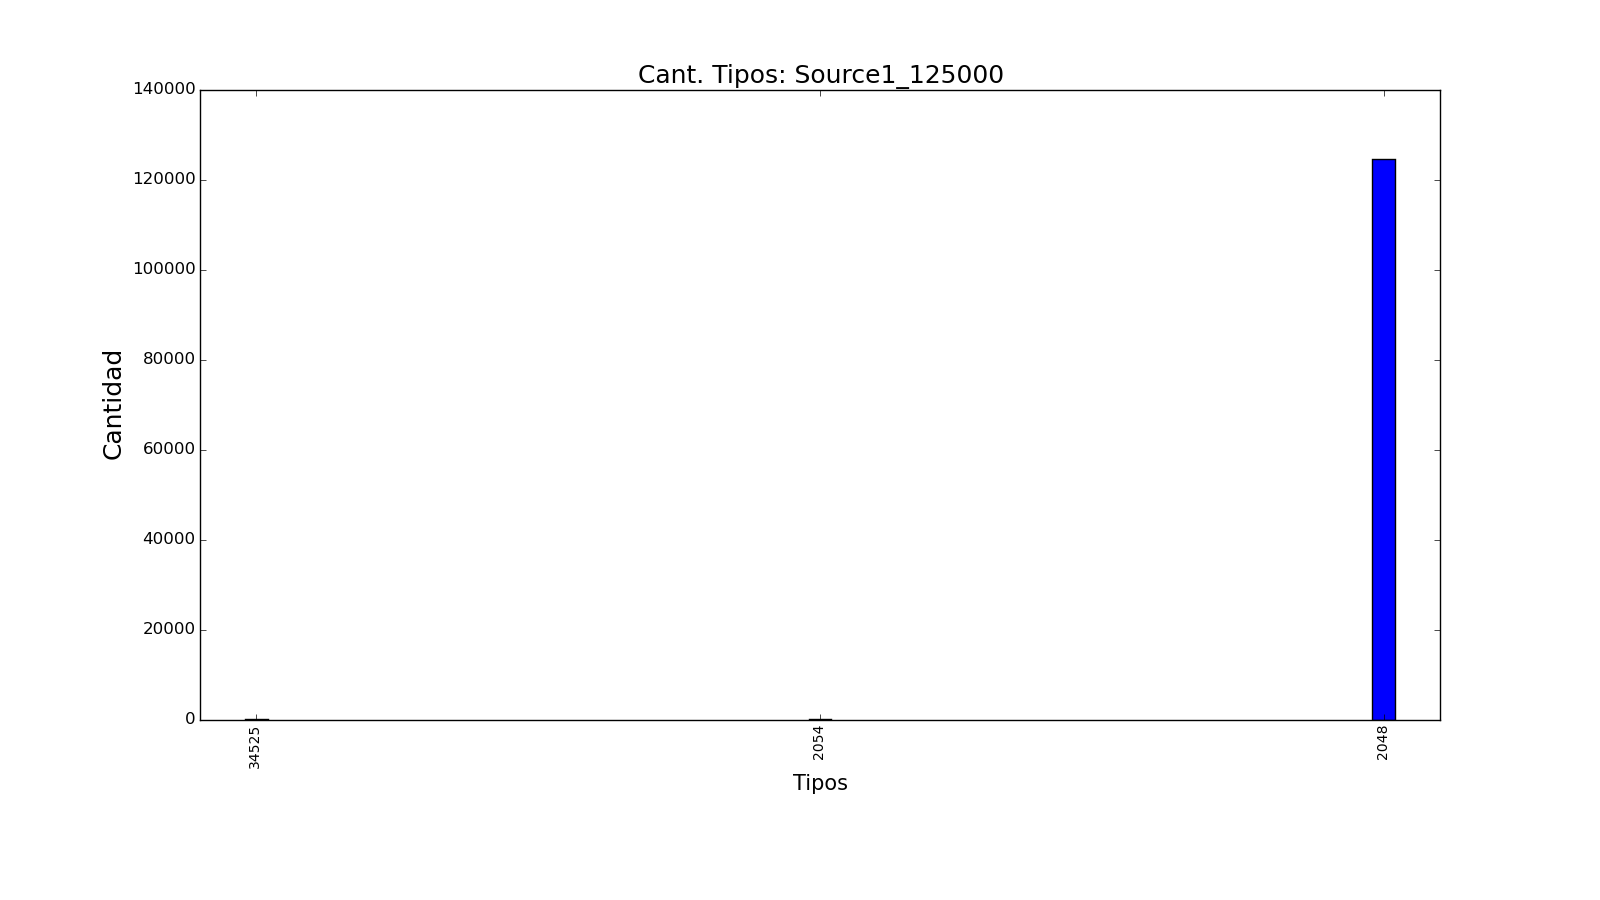
\includegraphics[width=1\textwidth]{../resultados/Casa/histogram_types.png}
       \caption{Protocolos de los paquetes capturados}
       \label{red-hogarena-types}
\end{figure}

\begin{figure}[H]
       \centering
       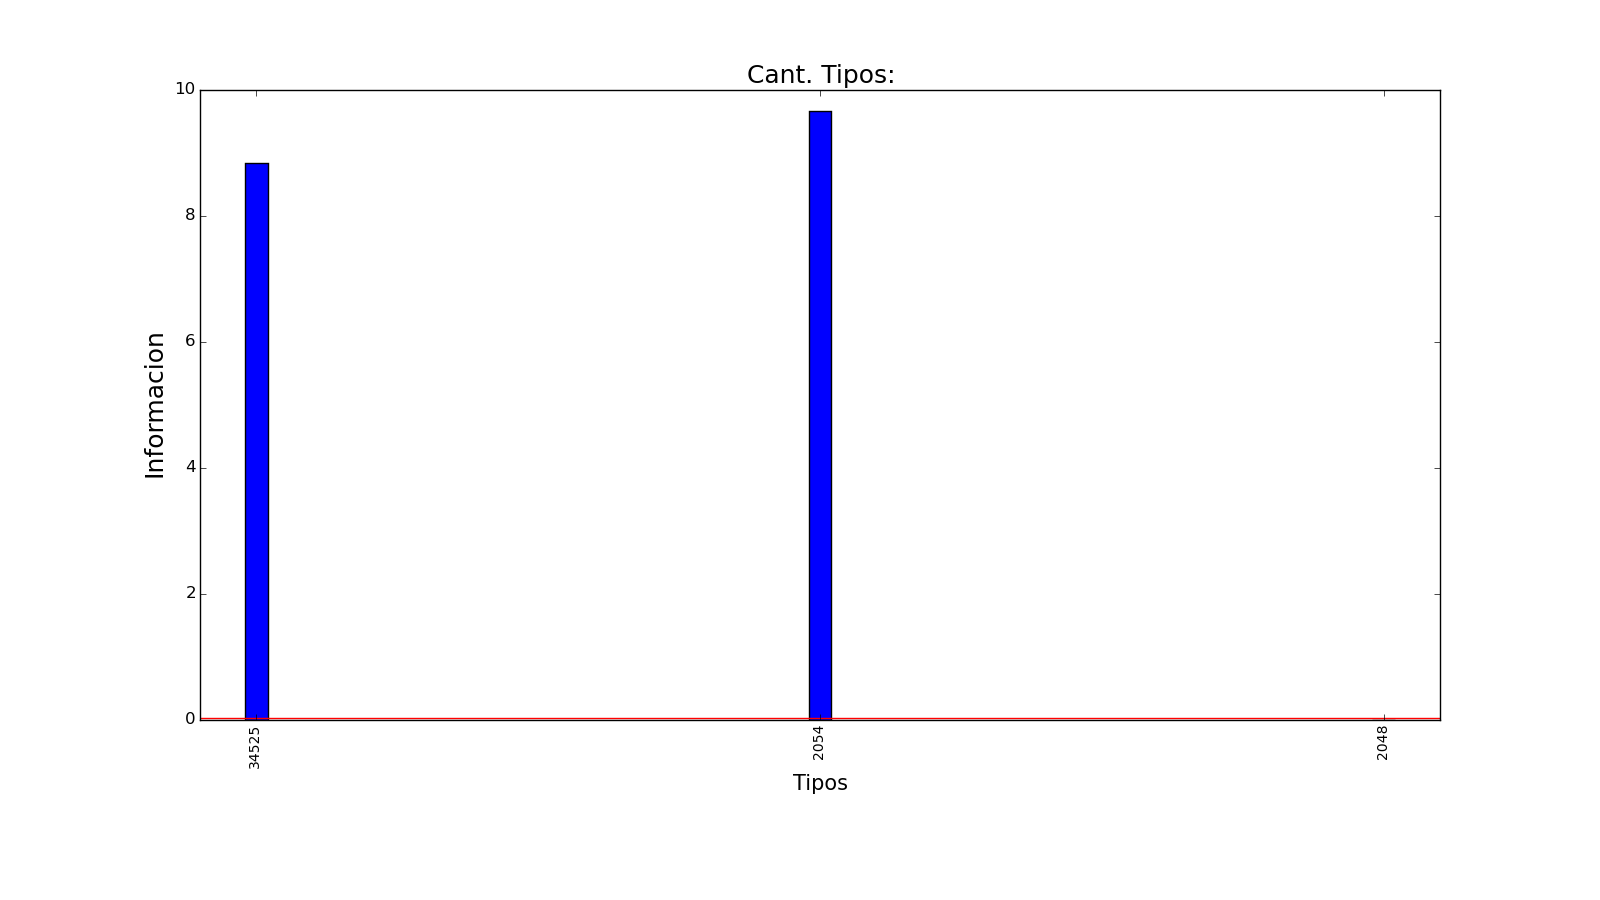
\includegraphics[width=1\textwidth]{../resultados/Casa/histogram_types_information.png}
       \caption{Información de los protocolos de los paquetes capturados}
       \label{red-hogarena-types-info}
\end{figure}


\begin{figure}[H]
       \centering
       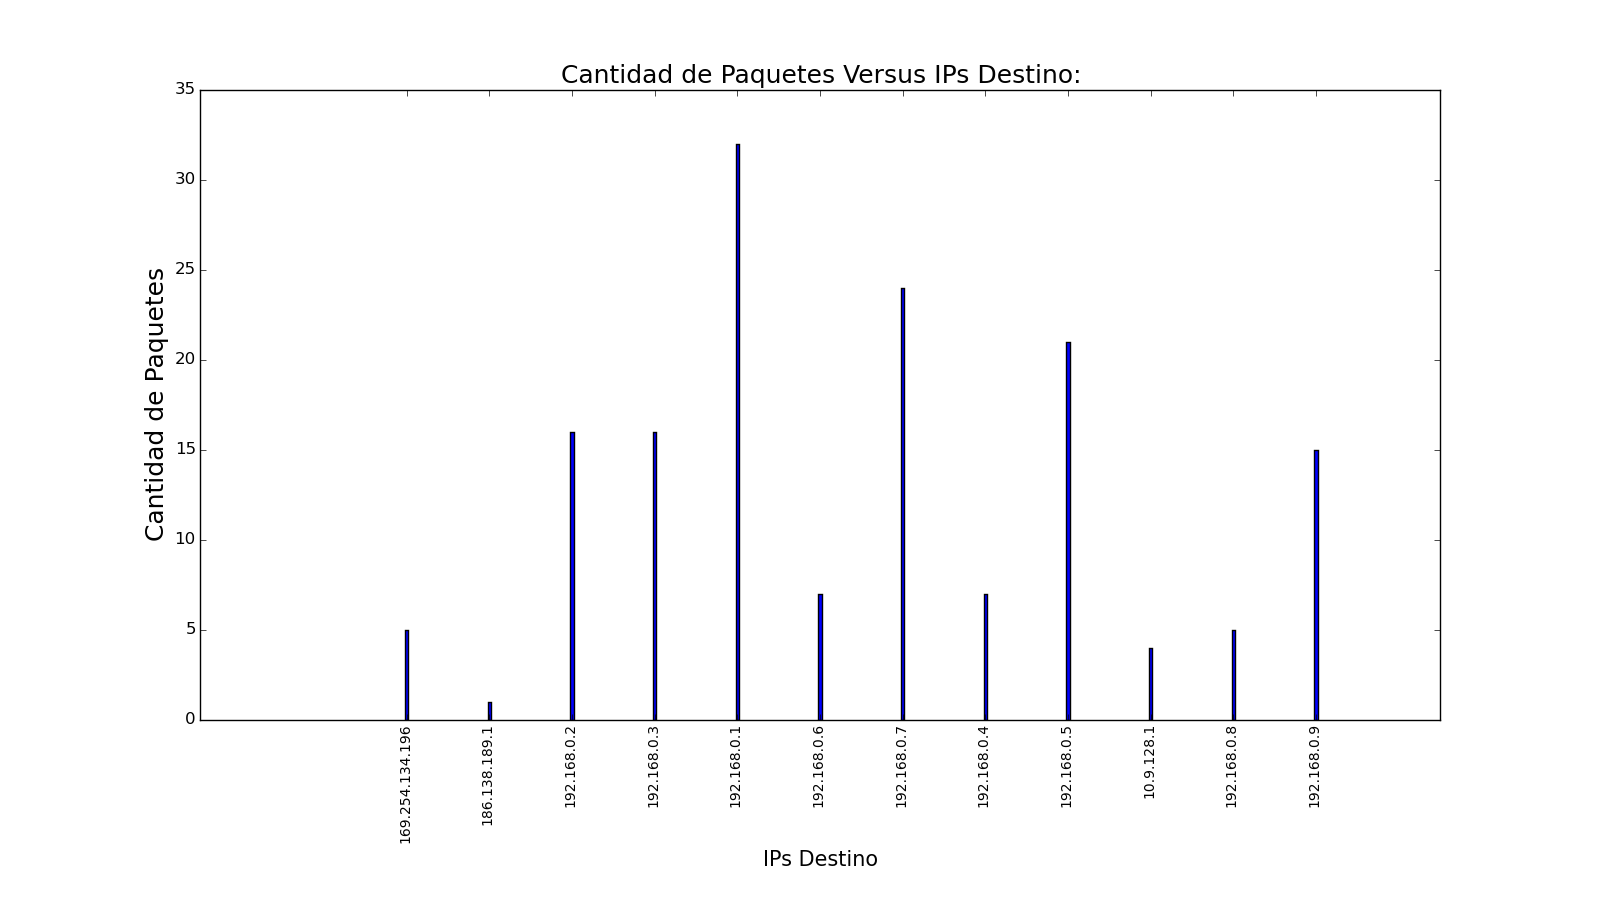
\includegraphics[width=1\textwidth]{../resultados/Casa/histogram_dst.png}
       \caption{IPs destino de los paquetes ARP}
       \label{red-hogarena-arp-destination}
\end{figure}

\begin{figure}[H]
       \centering
       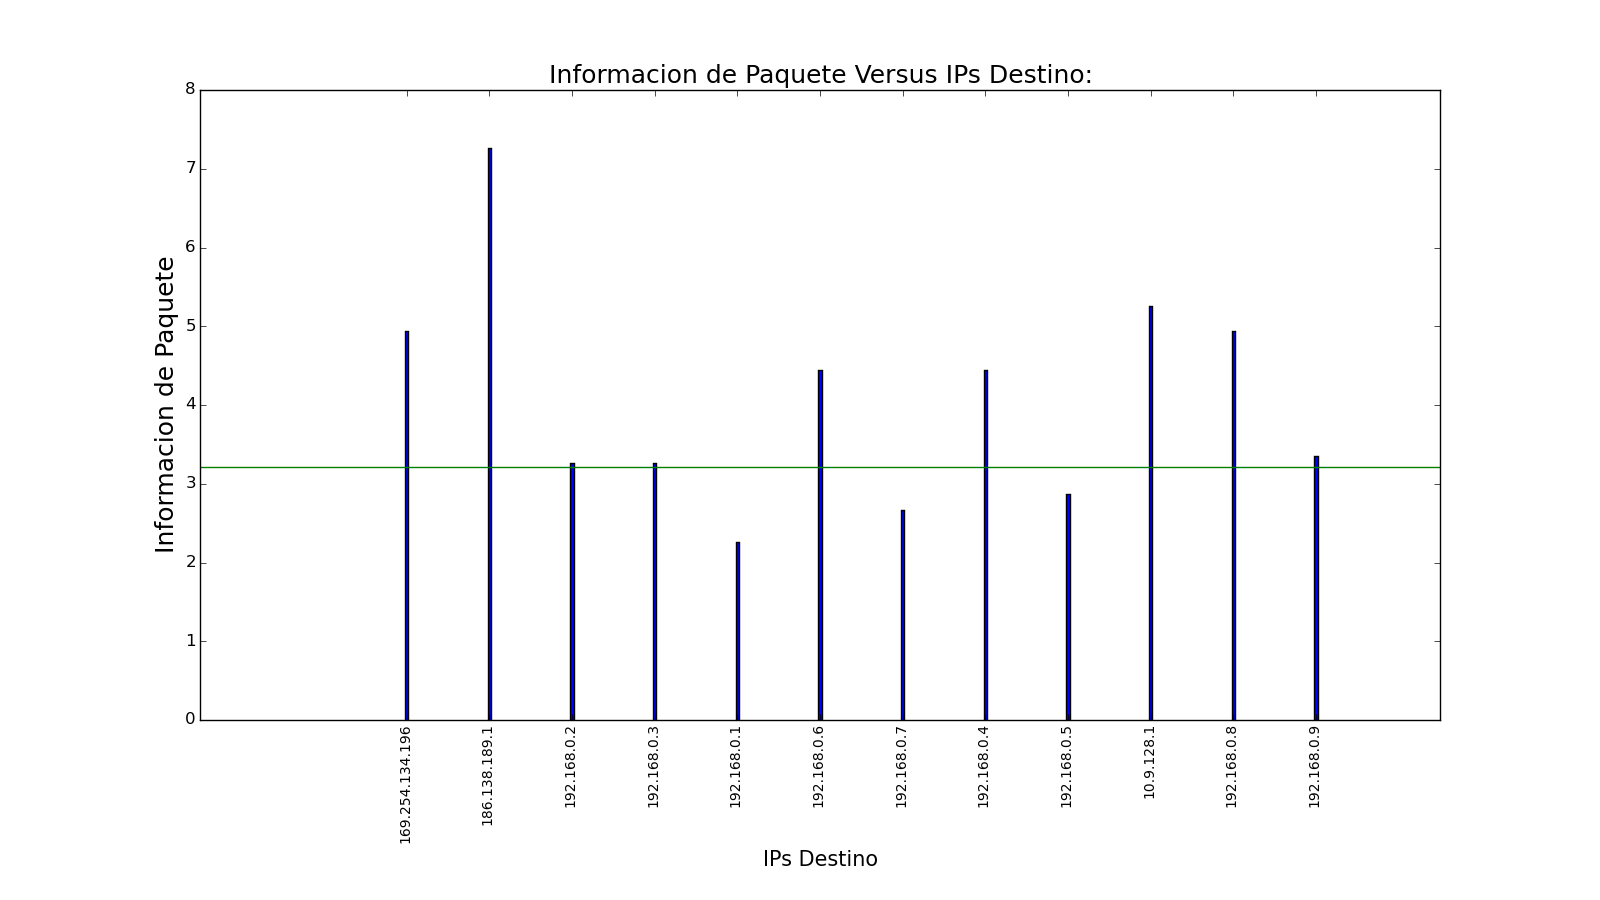
\includegraphics[width=1\textwidth]{../resultados/Casa/histogram_dst_information.png}
       \caption{Información de IPs destino de los paquetes ARP}
       \label{red-hogarena-arp-destination-info}
\end{figure}

\begin{figure}[H]
       \centering
       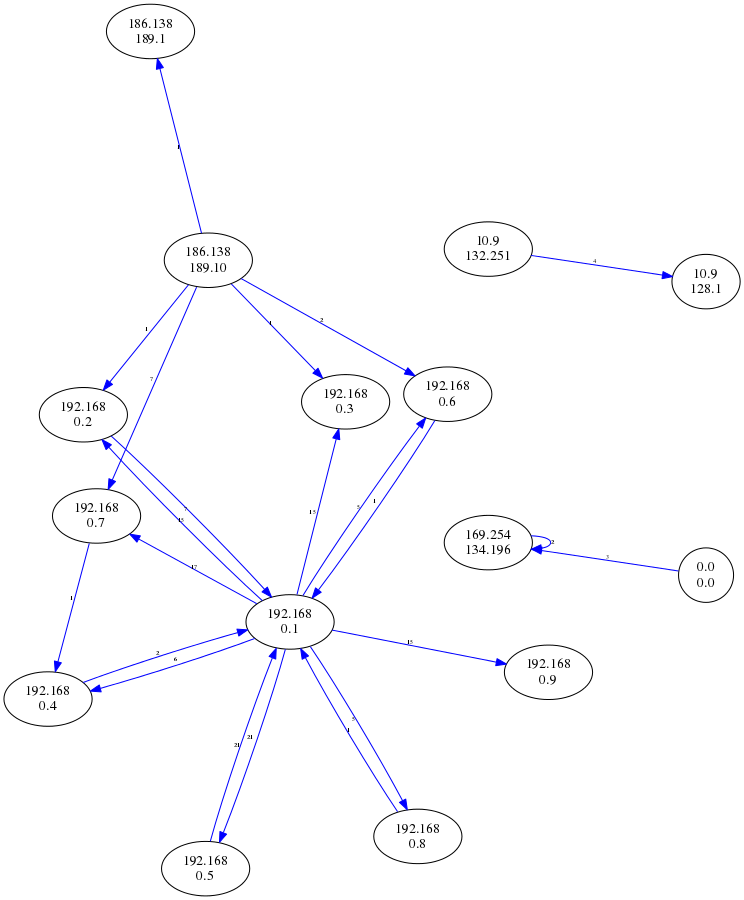
\includegraphics[width=1\textwidth]{../resultados/Casa/network.png}
       \caption{Tráfico de paquetes ARP}
       \label{red-hogarena-arp-traffic}
\end{figure}

